%! Licence = CC BY-NC-SA 4.0

%! Author = gianfluetsch
%! Date = 22. Jan 2022
%! Project = icth_summary

\section{Audiosignalen}

\subsection{Tonhöhenverschiebung von Audiosignalen}
\subsubsection{A}
Ein Audiosignal s(t) hat folgendes zweiseitiges Dichtespektrum S(f):

\begin{center}
    \vspace{-8pt}
    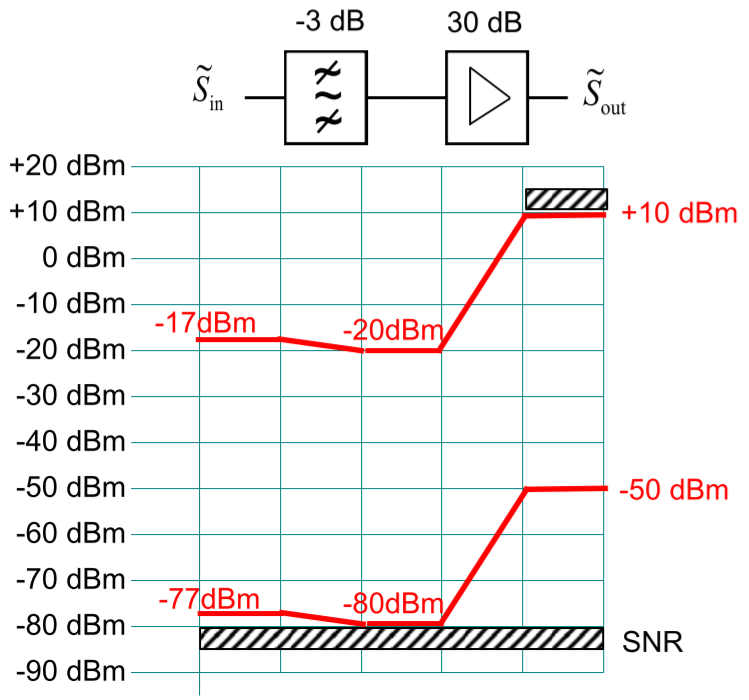
\includegraphics[width=.6\linewidth]{./13-audiosignale/hs2017}
    \vspace{-8pt}
\end{center}

Dieses Audiosignal s(t) wird nun mit einem Produktmodulator auf eine Trägerfrequenz von 8 kHz verschoben, so dass das untenstehende Spektrum resultiert:
\begin{center}
    \vspace{-8pt}
    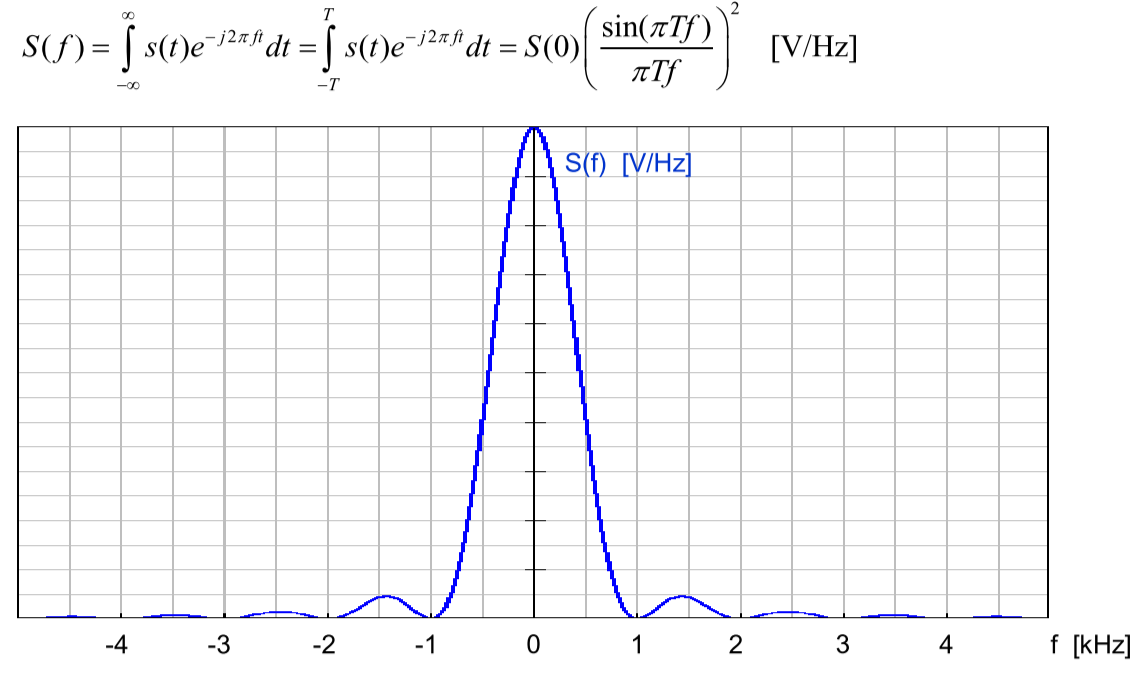
\includegraphics[width=.6\linewidth]{./13-audiosignale/hs2017_2}
    \vspace{-8pt}
\end{center}

Beschreiben Sie im Detail zwei Lösungen, die es erlauben, die Tonhöhe des Audiosignals um 200 Hz anzuheben (Mickey Mouse), so dass das untenstehende Ausgangsspektrum resultiert.
\begin{center}
    \vspace{-8pt}
    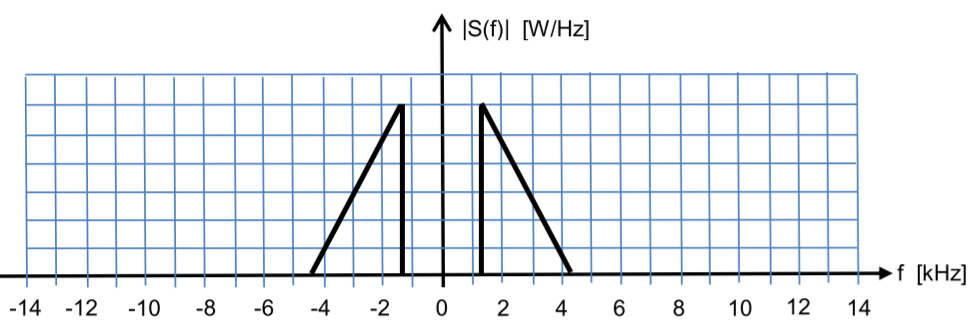
\includegraphics[width=.6\linewidth]{./13-audiosignale/hs2017_3}
    \vspace{-8pt}
\end{center}

\paragraph{Lösung 1}\mbox{}\\
\begin{itemize}
    \item Elimination des oberen Seitenbandes (USB) durch ein Tiefpassfilter mit der Grenzfrequenz 8 kHz
    \item Demodulation mit einer LO-Frequenz von 8200 Hz, welches das untere Seitenband (LSB) mit einem Frequenzshift von +200 Hz in das Basisband zurückschiebt
\end{itemize}

\paragraph{Lösung 2}\mbox{}\\
\begin{itemize}
    \item Elimination des unteren Seitenbandes (LSB) durch ein Hochpassfilter mit der Grenzfrequenz 8 kHz
    \item Demodulation mit einer LO-Frequenz von 7800 Hz, welches das obere Seitenband (USB) mit einem Frequenzshift von 1200 Hz in das Basisband zurückschiebt
\end{itemize}

\paragraph{Lösung 3}\mbox{}\\
\begin{itemize}
    \item Durch die Demodulation entsteht eine Spektrumskomponente bei der doppelten Trägerfrequenz von ca. 16 kHz
    \item Diese hörbaren Frequenzanteile können mit einem Tiefpassfilter eliminiert werden
\end{itemize}

\subsection{Abtastung von Audiosignalen}
\subsubsection{A}
Ein nichtperiodisches Audiosignal s(t) hat folgendes zweiseitiges Dichtespektrum S(f):
\begin{center}
    \vspace{-8pt}
    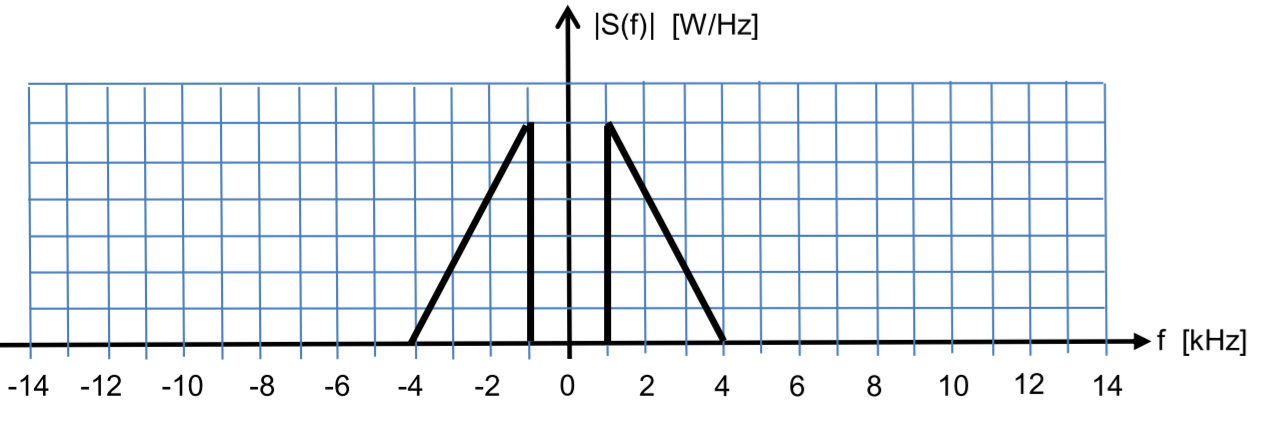
\includegraphics[width=.6\linewidth]{./13-audiosignale/hs2016}
    \vspace{-8pt}
\end{center}

Dieses Audiosignal s(t) wird nun mit einer Samplingfrequenz $f_s = 10 kHz$ abgetastet. Zeichnen Sie das resultierende zweiseitige Spektrum des abgetasteten Audiosignals in die
untenstehende Grafik ein:
\begin{center}
    \vspace{-8pt}
    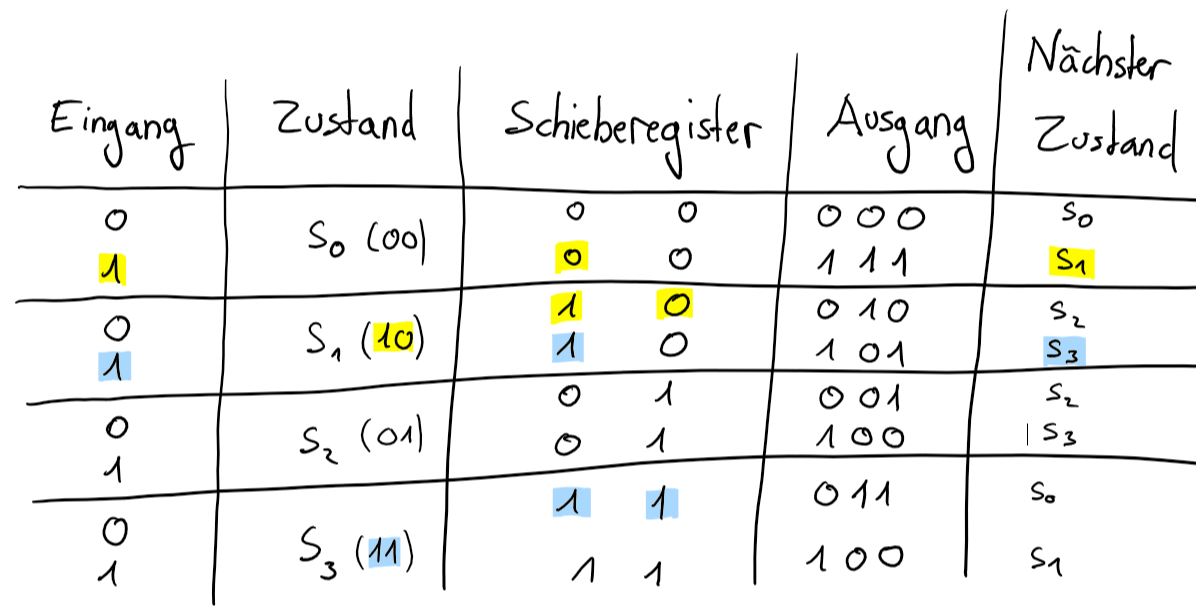
\includegraphics[width=.6\linewidth]{./13-audiosignale/hs2016_2}
    \vspace{-8pt}
\end{center}

\textbf{Tritt bei der Abtastfrequenz von $f_s = 10 kHz$ Aliasing auf?}\\
Nein es tritt kein Aliasing auf, da die höchste im Audiosignal vorkommende Frequenz von 4 kHz kleiner als die Hälfte der Abtastfrequenz $f_s/2 = 5 kHz$ ist und sich deshalb die periodischen Spektrumswiederholungen nicht überlappen.\\

Als Alternative wird das Audiosignal s(t) mit einer tieferen Samplingfrequenz $f_s = 7 kHz$ abgetastet. Zeichnen Sie das resultiererende zweiseitige Spektrum des abgetasteten Audio-
signals in die untenstehende Grafik ein:
\begin{center}
    \vspace{-8pt}
    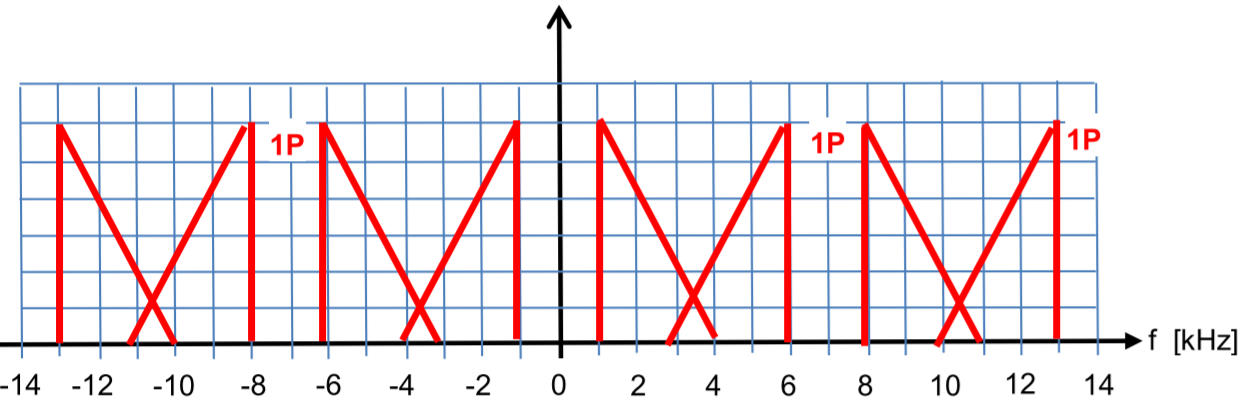
\includegraphics[width=.6\linewidth]{./13-audiosignale/hs2016_3}
    \vspace{-8pt}
\end{center}

\textbf{Tritt bei der Abtastfrequenz von $f_s = 7 kHz$ Aliasing auf?}\\
Ja es tritt Aliasing auf, da die höchste im Audiosignal vorkommende Frequenz von 4 kHz grösser als die Hälfte der Abtastfrequenz $f_s/2 = 3.5 kHz$ ist und sich deshalb die
periodischen Spektrumswiederholungen überlappen.\\

\textbf{Wie kann bei einer gegebenen Abtastfrequenz $f_s$ das Auftreten von Aliasing beim Abtasten vermieden werden?}\\
Durch Vorschalten eines Tiefpassfilters mit einer Grenzfrequenz $f_g < f_s/2$, so dass keine Spektrumsüberlappungen auftreten.